\documentclass[handout,10pt]{beamer}%

\usepackage{ucs}
\usepackage[utf8x]{inputenc}
\usepackage[T1]{fontenc}
\usepackage[ngerman]{babel}

\usepackage{bm}

\usepackage{xcolor}
\usepackage{tikz}
\usetikzlibrary{arrows}
\usetikzlibrary{positioning,automata}

\usepackage{algorithm}
\usepackage[noend]{algpseudocode}


% -----------

\algdef{SE}[DOWHILE]{Do}{doWhile}{\algorithmicdo}[1]{\algorithmicwhile\ #1}%

\newcommand{\MinAlg}{\textsc{MinimizeDFA}}
\newcommand{\CompUnr}{\textsc{FindUnreachables}}
\newcommand{\RemUnr}{\textsc{RemUnreachables}}
\newcommand{\CompDist}{\textsc{FindEquivPairs}}
\newcommand{\mCompDist}{\textsc{$m$-FindEquivPairs}}
\newcommand{\RemEq}{\textsc{RemEquivPairs}}

\newcommand{\mmD}{\mathfrak{D}}

\newcommand{\nSO}{{n_s}}
\newcommand{\nEQ}{{n_e}}
\newcommand{\nUN}{{n_u}}
\newcommand{\nF}{{n_F}}
\newcommand{\kAL}{k}

\newcommand{\A}{\mathcal{A}}
\newcommand{\Amin}{{\mathcal{A}_{min}}}

\newcommand{\gregorColor}{Violet}
\newcommand{\gregor}[1]{\textcolor{\gregorColor}{\textbf{Gregor:} #1}}

\newcommand{\x}{$\blacksquare$}

\setbeamertemplate{footline}[frame number]

% -----------

\title{Generation of DFA Minimization Problems}

\author{Gregor Sönnichsen}
\institute{Universität Bayreuth}
\subject{Bachelors Thesis}


\usetheme{default}
\usecolortheme{whale}
\definecolor{darkgreen}{RGB}{3,138,94}
\setbeamercolor{frametitle}{bg=darkgreen}
\setbeamercolor*{title}{bg=darkgreen, fg=white}
\setbeamertemplate{navigation symbols}{}

\bibliographystyle{plainurl}



\begin{document}
	
	\begin{frame}
		\titlepage
	\end{frame}
	
	% Introduction
	
	\section{Introduction}
	
	\begin{frame}
		\frametitle{Introduction}
		Automata theory is a classical topic in computer science curricula.
		
		Minimization of DFAs is a typical task for students:
		\begin{itemize}
			\item sufficiently easy to understand
			\item practical applications
			\item understanding can be tested easily
		\end{itemize}
		\vspace{0.3cm}
		Consequently, studying automatized generation of DFA minimization problems is interesting because it could\ldots
		\begin{itemize}
			\item \ldots free up precious time for exercise constructors
			
			(if a generator is implemented)
			\item \ldots yield a deeper insight
			
			in the nature of such problems
		\end{itemize}
	{\vspace{-2cm}\hfill
\includegraphics[width=0.2\linewidth]{zeitdiebe-besiegen-lebenszeit-gewinnen.jpg}\hspace{0.1cm}\tiny\footnotemark}
	
	\renewcommand{\footnotesize}{\tiny}
	
	{\footnotetext{\url{https://www.rindlerwahn.de/zeitdiebe-besiegen-und-mehr-lebenszeit-gewinnen}}}
	
	\end{frame}

	\begin{frame}
	\frametitle{Outline}
	\tableofcontents % [pausesections]
	\end{frame}
	
	% Thesis Content
	
	\section{Problem definition and approach}
	
	\begin{frame}
		\frametitle{Problem definition}
		\framesubtitle{Preliminaries (1/2)}
		
		A tuple $A = (Q, \Sigma, \delta, s, F)$ with $Q, \Sigma$ being a finite, $\delta \colon\ Q \times \Sigma \to Q$, $s \in Q$ and $F \subseteq Q$ is called \emph{deterministic finite automaton}.
		\vspace{0.3cm}
		
		% Note: Completeness
		
		We define the \emph{extended transition function} $\delta^* : Q \times \Sigma^* \to Q$ as:
		\begin{itemize}
			\item $\delta^*(q,\varepsilon) = q$
			\item $\delta^*(q,w\sigma) = \delta(\delta^*(q,w),\sigma)$ for all $q \in Q$, $w \in \Sigma^*$, $\sigma \in \Sigma$
		\end{itemize}
		\vspace{0.3cm}
		
		The \emph{language} of DFA is defined as $L(A) = \{\ w\ |\ \delta^*(w) \in F\ \}$.
		\vspace{0.3cm}
		
		We call a DFA \emph{minimal}, if there exists no other DFA with the same language having less states.
	\end{frame}
		
	\begin{frame}
		\frametitle{Problem definition}
		\framesubtitle{Preliminaries (2/2)}
		
		We say a state $q$ is \emph{unreachable}, iff there is no word $w \in \Sigma^*$ such that $\delta^*(s, w) = q$.
		\vspace{0.3cm}
		
		A state pair $q_1, q_2 \in Q$ is called \emph{equivalent}, iff $\sim_A(q_1, q_2)$ is true, where
		\begin{displaymath}
		q_1 \sim_A q_2\ \Leftrightarrow_{def}\ \forall z \in \Sigma^* \colon\ (\delta^*(q_1, z) \in F \Leftrightarrow \delta^*(q_2, z) \in F)
		\end{displaymath}
		
		\begin{example}
			\centering
			\begin{tikzpicture}[initial text={}]
			\tikzstyle{every state}=[minimum size=5mm, inner sep=0pt]
			
			\node[initial, state]  (0) at (0, 0) {$0$};
			
			\node[state]           (1) at (1.5,-1) {$1$};
			\node[state]           (2) at (1.5, 1) {$2$};
			
			\node[accepting,state] (3) at (3, 0) {$3$};
			
			\node[state]           (4) at (4.5,0) {$4$};
			
			\path[->]
			(0) edge node [above right]  {$a$} (1)
			(0) edge node [above left]  {$b$} (2)
			
			(1) edge node [above left=-0.1cm] {$a,b$} (3)
			(2) edge node [above right=-0.1cm] {$a,b$} (3)
			
			(3) edge [loop below] node [right] {$a,b$} (3)
			
			(4) edge node [above] {$a,b$} (3)
			;
			\end{tikzpicture}
		\end{example}
	
		\begin{theorem}
			A DFA is minimal, iff it has neither unreachable nor equivalent states.
		\end{theorem}
	\end{frame}


	\begin{frame}
		\frametitle{Problem definition}
		\framesubtitle{Hopcroft's Minimization Algorithm}
		
		\begin{tikzpicture}[remember picture,overlay]
		\node[xshift=-1.5cm,yshift=-3cm] at (current page.north east) {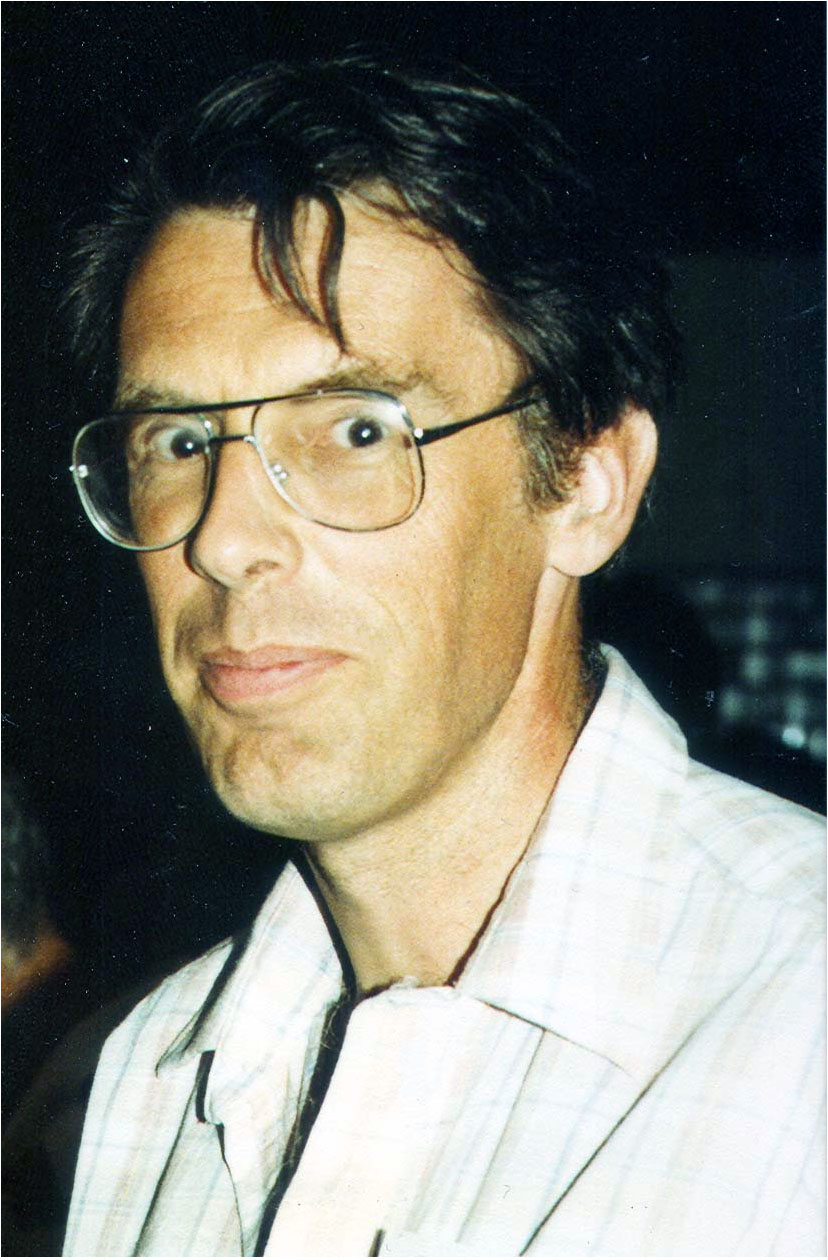
\includegraphics[height=2.5cm]{jehyoung.jpg}};
		\end{tikzpicture}
		
		\begin{enumerate}
		\item Compute all unreachable states
		\item Remove all unreachable states and their transitions
		\item Compute all inequivalent state pairs ($\not\sim_A$)
		\begin{algorithmic}[1]
			\Function{\CompDist}{$A$}
			\State $i \gets 0$
			\State $m(0) \gets \{ (p,q), (q,p)\ |\ p \in F, q \notin F \}$
			\Do
			\State $i \gets i + 1$
			\State $m(i) \gets \{ (p,q), (q,p)\ |\ (p,q) \notin \bigcup{m(\cdot)} \land$
			\State \hfill$\exists \sigma \in \Sigma \colon (\delta(p,\sigma), \delta(q,\sigma)) \in m(i-1) \}$
			\doWhile {$m(i) \neq \emptyset$}
			\State \Return $\bigcup{m(\cdot)}$
			\EndFunction
		\end{algorithmic}
		\item Merge all equivalent state pairs
		\end{enumerate}
	\end{frame}

	
	\begin{frame}
		\frametitle{Problem definition}
		\framesubtitle{A sample DFA minimization problem\ldots}
		{\raggedright\itshape \underline{Task:} Consider the below shown deterministic finite automaton $A$:}
		\begin{center}\resizebox{.75\linewidth}{!}{
				\begin{tikzpicture}[initial text={},scale=1., every node/.style={transform shape}]
				\tikzstyle{every state}=[minimum size=5mm, inner sep=0pt]
				
				\node[initial, state]  (0) at (0, 0)    {$0$};
				\node[state] 		   (1) at (6, 0)    {$1$};
				\node[state,accepting] (2) at (4,0)     {$2$};
				\node[state]           (3) at (2, -1.5) {$3$};
				\node[state,accepting] (4) at (4,-3)    {$4$};
				\node[state]           (5) at (4,-1.5)  {$5$};
				\node[state]           (6) at (2,0)     {$6$};
				
				\path[->]
				(0) edge node [above=-0.07cm]  {$a$}   (6)
				(0) edge [bend left] node [above=-0.07cm]  {$b$}   (2)
				
				(1) edge node [above=-0.07cm]  {$a$}   (2)
				(1) edge node [below right=-0.15cm]  {$b$}   (4)
				
				(2) edge [bend left] node [above=-0.07cm]  {$a$}   (1)
				(2) edge node [below right=-0.15cm]  {$b$}   (3)
				
				(3) edge node [left=-0.07cm]  {$a$}   (6)
				(3) edge node [above right=-0.15cm]  {$b$}   (4)
				
				(4) edge [bend right] node [below right=-0.15cm]  {$a$}   (1)
				(4) edge [bend left] node [below left=-0.15cm]  {$b$}   (0)
				
				(5) edge node [below right=-0.15cm]  {$a$}   (1)
				(5) edge node [left=-0.07cm]  {$b$}   (4)
				
				(6) edge [bend right] node [below=-0.07cm]  {$a$}   (1)
				(6) edge node [above=-0.07cm]  {$b$}   (2)
				;
				\end{tikzpicture}
		}\end{center}
		{\itshape Apply the minimization algorithm and illustrate for each state pair of $A$ during which \CompDist-iteration it was marked. Draw the resulting automaton.}
		
	\end{frame}


	\begin{frame}
		\frametitle{Problem definition}
		\framesubtitle{\ldots and its solution}
	
		{\raggedright\itshape \underline{Solution:}\newline
			Step 1: Detect and eliminate unreachable states.
			\begin{tabbing}
				\qquad\textnormal{State $5$ is unreachable.}
			\end{tabbing}
			Step 2: Apply \CompDist\ to $A$ and merge equivalent state pairs:\par
		}
		\begin{columns}
		\begin{column}{.4\textwidth}
			\vspace{0.5cm}
			\qquad
			\begin{tabular}{c|c|c|c|c|c|c}
				& 0  & 1  & 2  & 3  & 4  & 6  \\\hline
				0 & \x & 1  & 0  &    & 0  & 2  \\\hline
				1 & \x & \x & 0  & 1  & 0  & 1  \\\hline
				2 & \x & \x & \x & 0  &    & 0  \\\hline
				3 & \x & \x & \x & \x & 0  & 2  \\\hline
				4 & \x & \x & \x & \x & \x & 0  \\\hline
				6 & \x & \x & \x & \x & \x & \x \\
			\end{tabular}
		\end{column}
		\begin{column}{.5\textwidth}\centering\resizebox{1.\linewidth}{!}{
			\begin{tikzpicture}[initial text={},scale=1., every node/.style={transform shape}]
			\tikzstyle{every state}=[minimum size=5mm, inner sep=0pt]
			
			\node[initial, state]  (03) at (0, 0)   {$03$};
			\node[state] 		   (1) at (6, 0)   {$1$};
			\node[state,accepting] (24) at (4,0)    {$24$};
			\node[state]           (6) at (2,0)    {$6$};
			
			\path[->]
			(03) edge node [above=-0.07cm]  {$a$}   (6)
			(03) edge [bend left] node [above=-0.07cm]  {$b$}   (24)
			
			(1) edge node [above=-0.13cm]  {$a,b$}   (24)
			
			(24) edge [bend left=50] node [above=-0.07cm]  {$a$}   (1)
			(24) edge [bend right=50] node [above=-0.07cm]  {$b$}   (03)
			
			(6) edge [bend right] node [below=-0.07cm]  {$a$}   (1)
			(6) edge node [above=-0.07cm]  {$b$}   (24)
			;
			\end{tikzpicture}
		}\end{column}
		\end{columns}
	\end{frame}

	\begin{frame}
		\frametitle{Problem Definition and Approach}
		Problem: How to generate a \emph{DFa Minimization Problem} $(A_{sol}, A_{task})$?
		
		\vspace{0.2cm}
		Idea: First generate $A_{sol}$, then add equivalent, then unreachable states.
		
		$\Rightarrow$ modular pipeline architecture
		
		\vspace{0.4cm}
		\begin{tikzpicture}[initial text={}, every node/.style={transform shape}]
		
		\node[draw,style={rounded corners}] (p) at (0,0) {$\nSO, \kAL, \nF, d, p_{sol}, p_{task}, \nEQ,\nUN, c$};
		
		\node[draw] (1) at (0,-2) {
			\begin{minipage}{\linewidth}
			Generate DFA Minimization Problem
			
			\begin{itemize}
				\item Generate Minimal DFA
				
				\qquad (using a rejection algorithm and randomization/enumeration)
				
				\item Extend Minimal DFA
				\begin{itemize}
					\item Add Equivalent States
					\item Add Unreachable States
				\end{itemize}
			\end{itemize}
			
			\end{minipage}
		};
	
		\node[draw,style={rounded corners}] (o) at (0,-4) {$A_{sol}, A_{task}$};
		
		\path[->]
		(p) edge (1)
		(1) edge (o)
		;
		\end{tikzpicture}
		
	\end{frame}

	\begin{frame}
	\frametitle{Outline}
	\tableofcontents % [pausesections]
	\end{frame}
	
	
	\section{Generating Minimal DFAs}
	
	\begin{frame}
		\frametitle{Generating Minimal DFAs}
		\framesubtitle{Rejection Algorithm}
		Approach: Generate test DFAs until they match the demanded properties.
		
		\vspace{0.2cm}
		\begin{algorithmic}[1]
			\Function{GenNewMinDFA\ }{$\nSO, \kAL, \nF, d, p$}
			
			\vspace{0.2cm}
			
			\State $l \gets$ all DFAs in DB$_{found}$ matching $\nSO, \kAL, \nF$
			
			\vspace{0.2cm}
			
			\While {True}
			
				\vspace{0.2cm}
				
				\State generate DFA $A_{test}$ with $|Q|, |\Sigma|, |F|$ matching $\nSO, \kAL, \nF$
	
				\vspace{0.2cm}
				
				\If {$A_{test}$ not minimal \textbf{or} $d \neq \mmD(A_{test})$}
					\State \textbf{continue}
				\EndIf
				
				\If {$p = 1$ \textbf{and} $A_{test}$ is not planar}
					\State \textbf{continue}
				\EndIf
				
				\If {$A_{test}$ is isomorph to any DFA in $l$}
					\State \textbf{continue}
				\EndIf
				
				\vspace{0.2cm}
				
				\State save $A_{test}$ and its respective properties in DB$_{found}$
				\State\Return $A_{test}$
			
			\EndWhile
			\EndFunction
		\end{algorithmic}
	
		\begin{tikzpicture}[remember picture,overlay]
		\node[xshift=-1.5cm,yshift=-6.25cm] at (current page.north east) {
\includegraphics[height=1.75cm]{rejection.jpg}};
		\end{tikzpicture}
	
	\end{frame}

	\begin{frame}
		\frametitle{Generating Minimal DFAs}
		\framesubtitle{Test DFA Generation}
		We will restrict ourselves to the following DFAs:
		\[
			Q = \mathbb{N}_0^ {\nSO-1}, \Sigma = \mathbb{N}_0^{\kAL-1}, s = 0
		\]
		
		\begin{enumerate}
			\item[(a)] Generation by Randomization:
			\begin{align*}
			F &= random\_subset(Q)\\
			\delta(q, \sigma) &= choose\_one(Q) \qquad\qquad \forall q\in Q, \sigma\in\Sigma
			\end{align*}
			
			\item[(b)] Generation by Enumeration:\\$ $\\
			An \emph{enumeration state} $s_{\nSO, \kAL, \nF} = (F_F,F_\delta)$ consists of two arrays of length $\nSO, \nSO*\kAL$, respectively.
			\begin{align*}
			F_F[i] = 1 &\Leftrightarrow_{def} i \in F\\
			F_\delta[i * \kAL + j] = q &\Leftrightarrow_{def} \delta(i, j) = q
			\end{align*}
		\end{enumerate}
	
	\end{frame}

	\begin{frame}
		\frametitle{Generating Minimal DFAs}
		\framesubtitle{Incrementing Enumeration States}
		Short demo how the associated DFA changes, when an enumeration state is incremented
	
	\end{frame}
	
	
	\begin{frame}
		\frametitle{Outline}
		\tableofcontents % [pausesections]
	\end{frame}
	
	\section{Extending Minimal DFAs}

	\begin{frame}
		\frametitle{Extending Minimal DFAs}
		\framesubtitle{Adding Equivalent States (1)}
		%	
		%		Reminder: Two states $q_1, q_2 \in Q$ are called \emph{equivalent} ($q_1 \sim_A q_2$), iff $\forall z\in\Sigma^* (\delta^ *(q_1, z) \in F \Leftrightarrow \delta^*(q_2, z) \in F)$.
		%	
		%		\vspace{0.2cm}
		Let the added states be $r_1,\ldots,r_\nEQ$, such that $Q_{re} = Q_{sol} \cup \{r_1,\ldots,r_\nEQ\}$ and each of the added states is equivalent to a distinct state in $Q_{re}$.
		
		\vspace{0.2cm}
		Observation: Each $r_i$ will be equivalent to a state $e$ of $A_{sol}$:
		\[
		\forall i \in [1,\nEQ] \colon\ \exists e \in Q_{sol}\colon\ r_i \sim_A e
		\]
		We will first choose an $e\in Q_{sol}$ for each state $r_i$ we create, then we add its transitions.
	
	\end{frame}

	\begin{frame}
		\frametitle{Extending Minimal DFAs}
		\framesubtitle{Adding Equivalent States (2)}
		
		Outgoing transitions. Observation:
		\begin{itemize}
			\item[] $r_i \sim_A e$
			
			\item[$\Rightarrow$] $\forall \sigma \in \Sigma \colon [\delta(r_i, \sigma)]_{\sim_A} = [\delta(e, \sigma)]_{\sim_A}$
		\end{itemize}
	
		\vspace{0.2cm}
		We see that $\delta(r_i, \sigma) = q$ must be in the same equivalency class as $\delta(e, \sigma) = p$.
		
		\vspace{0.2cm}
		Consequently:
		\begin{itemize}
			\item[R1:] For each symbol $\sigma \in \Sigma$ choose exactly one state $q\in[\delta(e, \sigma)]_{\sim_A}$ and set $\delta(r_i, \sigma) = q$.
		\end{itemize}
	
		\vspace{0.2cm}
		The rule is always fulfillable:
		\begin{itemize}
			\item $A_{sol}$ is complete
			\item every $r_i$ gets an out. transition for every alphabet symbol
		\end{itemize}
	
	\end{frame}

	\begin{frame}
	\frametitle{Extending Minimal DFAs}
	\framesubtitle{Adding Equivalent States (3)}
	
	Showcase how a to add outgoing transitions of an equivalent state
	
	\end{frame}

	\begin{frame}
		\frametitle{Extending Minimal DFAs}
		\framesubtitle{Adding Equivalent States (4)}
		
		Ingoing transitions. Observations:
		
		\vspace{0.2cm}
		\begin{itemize}
			\item $r_i$ must be reachable $\Rightarrow in(r_i) >= 1$
		\end{itemize}
	
		\vspace{0.2cm}
		Let $q$ be a state that gets an in. transition to $r_i$.
		
		\vspace{0.2cm}
		\begin{itemize}
			\item[] $q$ must remain in its equivalence class
			
			\item[$\Rightarrow$] $q$ has to have a transition to some state in $[r_i]_{\sim_A} = [e]_{\sim_A}$
			
			\item[$\Rightarrow$] given $\delta(q, \sigma) = p$ and $p \in [e]_{\sim_A}$, we can set $\delta(q, \sigma) = r_i$
		\end{itemize}
		
		\vspace{0.2cm}
		We see that $p$ must have at least $2$ ingoing transitions.
		
		\vspace{0.2cm}
		\begin{itemize}
			\item[R2:] Choose at least one $((q, \sigma), p) \in \delta$ with $[p] = [e]$ and $out(p) \geq 2$. Remove $((q, \sigma), p)$ from $\delta$ and add $((q, \sigma), r_i)$.
		\end{itemize}
	
		\vspace{0.2cm}
		General requirement regarding the choice of a state $e$ for an $r_i$: 
		\[
			duplicatable(q) \Leftrightarrow_{def} (\exists p \in [q]_{\sim_A}\colon out(p) \geq 2)
		\]
	
	\end{frame}

	\begin{frame}
		\frametitle{Extending Minimal DFAs}
		\framesubtitle{Adding Equivalent States (5)}
		
		Showcase how a to add ingoing transitions of an equivalent state
	
	\end{frame}

	\begin{frame}
		\frametitle{Extending Minimal DFAs}
		\framesubtitle{Adding Unreachable States}
	
		Reminder: We say a state $q$ is \emph{unreachable}, iff there is no word $w \in \Sigma^*$ such that $\delta^*(s, w) = q$.
		\vspace{0.3cm}
	
		\begin{algorithmic}[1]
			\Function{AddUnrStates\ }{$A, \nUN, c$}
			\State $U \gets \emptyset$
			\vspace{0.2cm}
			
			\For {$\nUN$ \textbf{times}}
				\vspace{0.2cm}
				
				\State let $q$ be the new state
				\vspace{0.2cm}
				
				\State add ingoing tr.\ from a random subset of $U\times\Sigma$
				\vspace{0.2cm}
				
				\State $\Sigma' \gets \textbf{if } c = 1 \textbf{ then } \Sigma \textbf{ else}$ random subset of $\Sigma$
				\State add outgoing tr.\ to $|\Sigma'|$ random states
				\vspace{0.2cm}
				
				\State add $q$ to $U$
			\EndFor
			\vspace{0.2cm}
			
			\State \Return $A$
			\EndFunction
		\end{algorithmic}
%	
%		\begin{tikzpicture}[remember picture,overlay]
%		\node[xshift=-1.5cm,yshift=-7.5cm] at (current page.north east) {
\includegraphics[height=1.75cm]{Fix-err-address-unreachable.jpg}};
%		\end{tikzpicture}
	
	\end{frame}

	\begin{frame}
	\frametitle{Outline}
	\tableofcontents % [pausesections]
	\end{frame}

	\section{Live Demonstration}
	
	\begin{frame}
		\frametitle{Live Demonstration}
		\framesubtitle{Program Architecture}
		\centering
	    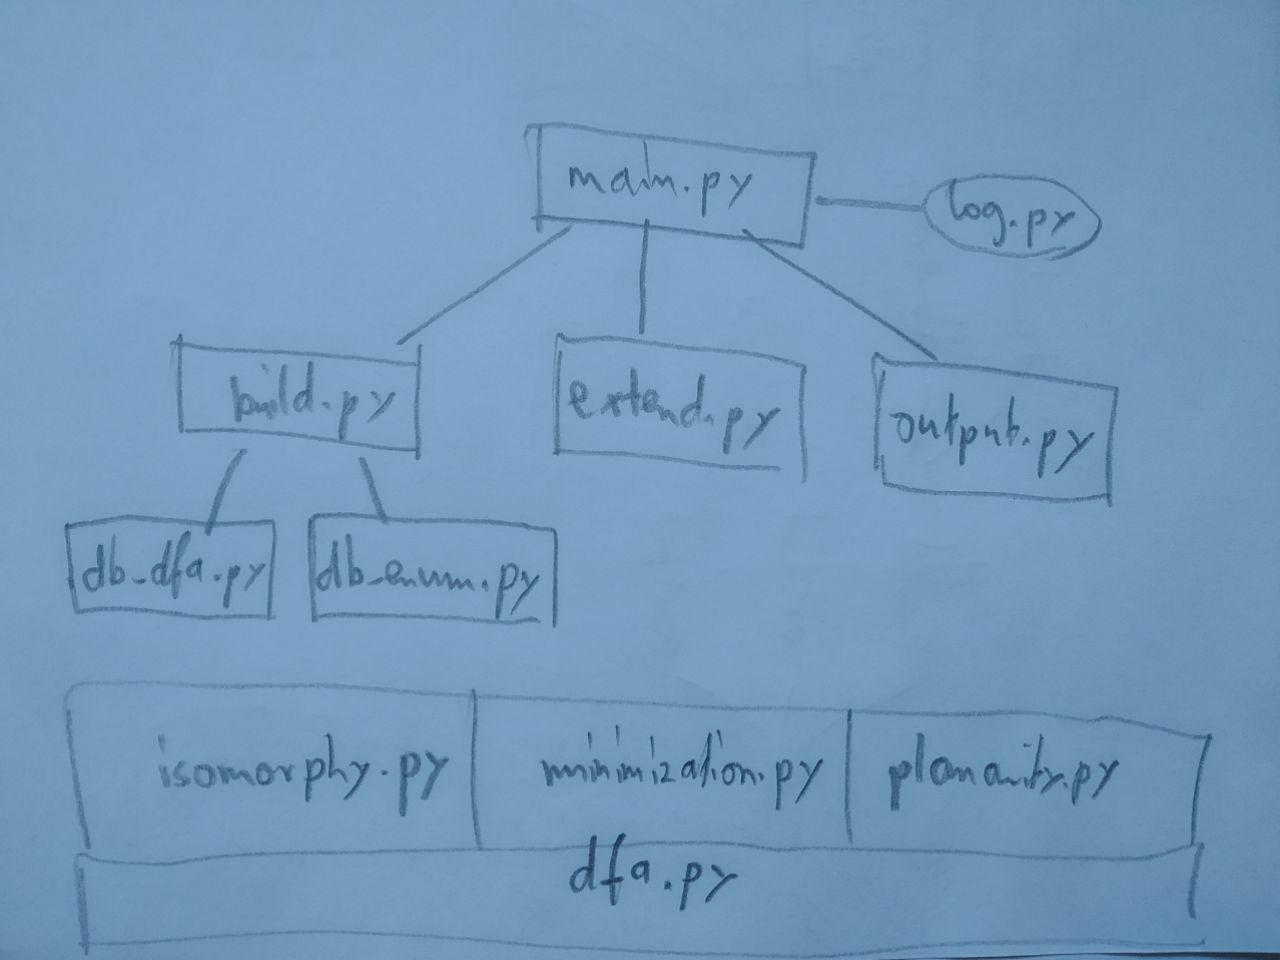
\includegraphics[width=0.9\linewidth]{prog_arch.jpg}
	
	\end{frame}

	\begin{frame}
		\frametitle{Live Demonstration}
		\framesubtitle{Command-Line Options}
		
		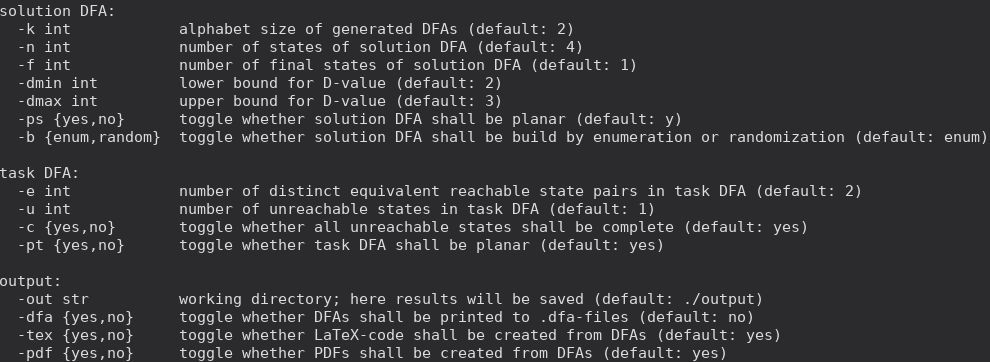
\includegraphics[width=\linewidth]{options.jpg}
	
	\end{frame}
	
	\section{Conclusion}

	\begin{frame}
		\frametitle{Conclusion}
		
		This presentation has\ldots
		\begin{itemize}
			\item introduced the problem of DFA Minimization Problem Generation
			\item given an overview over a possible solution
			\item shown that the theoretic results might be useful in praxis
		\end{itemize}
		Lookout:
		\begin{itemize}
			\item more parameters, ranged parameters
			
			The \emph{degree} of a state $q$ is defined as $deg(q) = d^-(q) + d^+(q)$.
			
			$\Rightarrow$ capping the max.\ degree?
			
			\item investigate planarity and drawing algorithms deeper
			\item complexity analysis
		\end{itemize}
	
	\end{frame}

	\begin{frame}
		\frametitle{References}
		
		\tiny
		\bibliography{presentation}
		
	\end{frame}

\end{document}

